\chapter{Results and Performance}
%
The generation of the data from the calibrated time series, i.e. the direct
detector response on air-shower photons, is what differs the PhotonStream data
from previous data representations. By finding single photons the goal is to
neglect the noise that is intrinsic when integrating over time series and
getting a more accurate time information. However, the results of this procedure
yield a different data set, so it is important to investigate the differences.

\section{Photon Extraction}
\label{sec:ph_ex}%
%
The photon extraction is the key difference when generating PhotonStream data.
It does not calculate the photon features from the time series but aims at
finding the single photon pulses, which opens the possibility of generating
arrival times per photon and hopefully yields an accurate description of the
air-showers. When comparing the PhotonStream data to the standard data
representation, the intuitive questions at hand are:
%
\begin{enumerate}
  \item What is the difference concerning the number of reconstructed photons?
  \item What is the difference in the number of noise photons?
  \item What is the difference between simulations and data?
\end{enumerate}
%
To answer these questions the images for specific events generated by the
photon extraction can be compared to the standard LP images. In
\autoref{fig:difference} and \autoref{fig:difference2} different data events
from a single run are shown for both data representations. The top camera image
shows the PE as generated by the photon extractor for the PhotonStream. The
bottom image shows the PE as generated from the LP of the time series. The
middle image shows the difference of both images in PE per pixel.

For those four example events a clear picture evolves: The difference between
both images is nearly always positive, meaning the photon extractor is
generally finding more photons in the time series. Furthermore, the biggest
differences lie within the air-shower pixels. So it seems that the difference
is dependant on the brightness, i.e. the photon extractor generates a bigger
PE difference for very bright pixels. Lastly, the difference in noise pixels is
very close to zero with small deviations in both directions.

Apart from these deviations, the PhotonStream data frequently contains a small
cluster of photons a few pixel rows above the camera center (e.g. in event 51,
\autoref{fig:difference}). These photons are not found in LP data. When
observing the Crab Nebula there is another bright star in the field of view of
the telescope: [NAME]. The light of this star is causing the bright spots in
the PhotonStream data. These spots are not visible in the LP data, because
it only contains a small time frame around the largest pulse, i.e. the
air-shower. This way, there is only a small part of the star's light present in
the event, which is not enough to significantly differ it from background
light. Luckily, the DBSCAN clustering intrinsically does not classify these
photons as air-shower photons. The space-time topology of a steady but faint
source apparently does not suit the clustering criteria.
%
\begin{figure}
  \subcaptionbox{Semi-logarithmic normalized distribution.\label{fig:pe_diffs_log}}[0.5\textwidth]{
    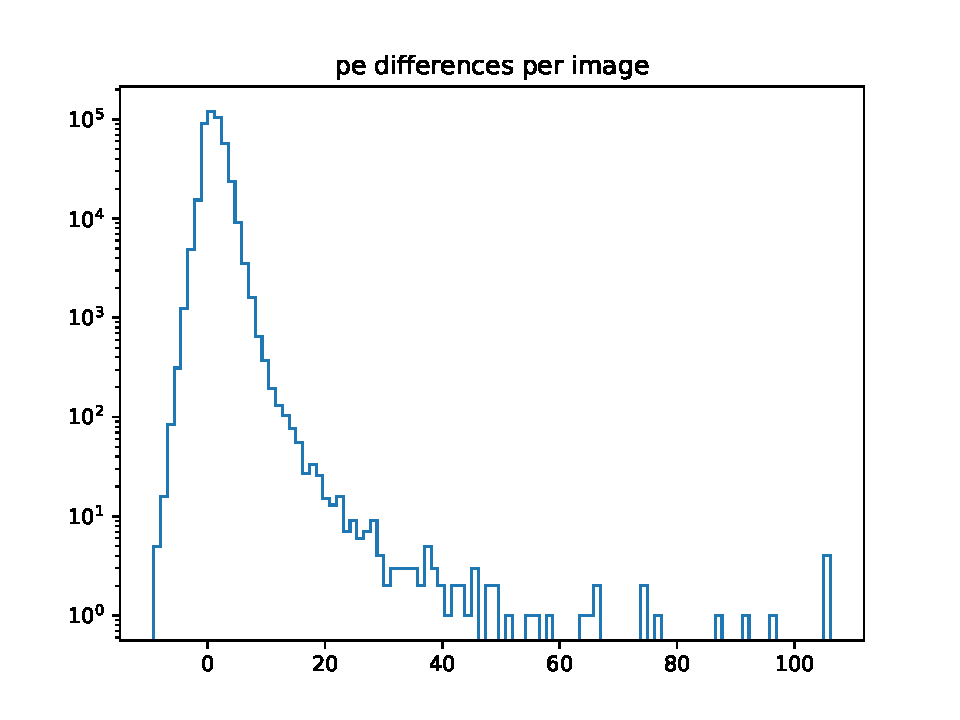
\includegraphics[width=0.5\textwidth]{Plots/diffs_hist_DBSCAN_pe_20131104_162_logy.pdf}
  }
  \subcaptionbox{Normalized distribution.\label{fig:pe_diffs}}[0.5\textwidth]{
    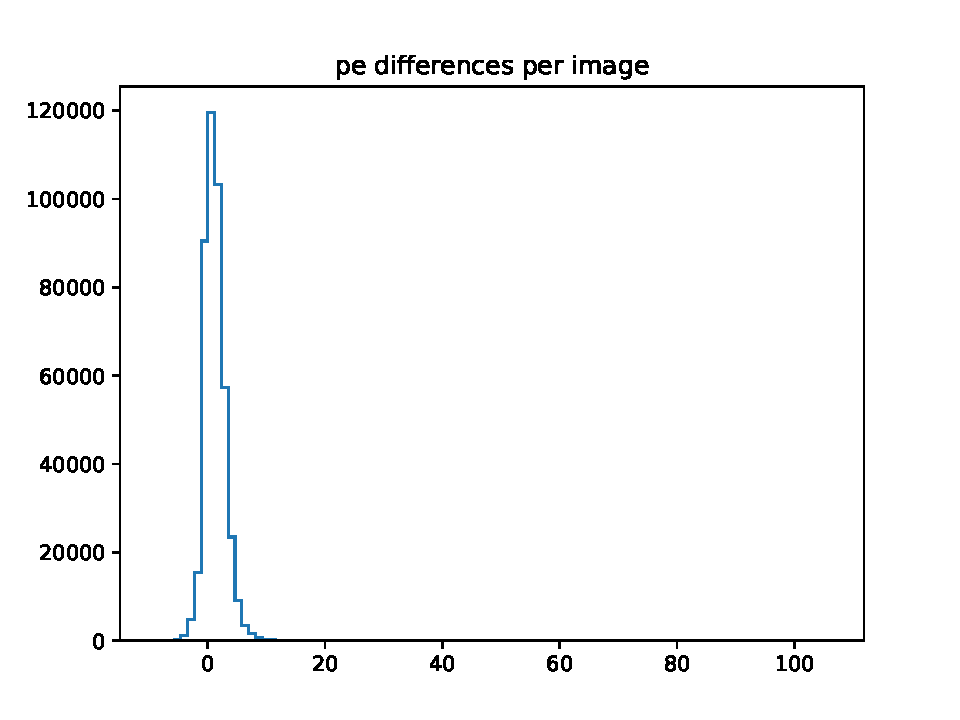
\includegraphics[width=0.5\textwidth]{Plots/diffs_hist_DBSCAN_pe_20131104_162.pdf}
  }
  \caption{PE differences per event and pixel between LP data and PhotonStream data accumulated for 300 events and normalized.}
  % \label{fig:pe_diffs}
\end{figure}
%

\autoref{fig:pe_diffs} shows the distribution of the PE differences as
described above accumulated for 300 events. The PhotonStream data on average contains
aorund 2 PE more than the corresponding LP event. However, as is visible in
\autoref{fig:pe_diffs_log} there is quite a number of pixels deviating by up to
20 PE. This reflects the observations from the four example events discussed
above: the majority of pixels contains one to two PE more than the PhotonStream
data while the few shower pixels contain a larger amount of PE more than the LP
data.


%
\begin{figure}
  \begin{subfigure}{0.5\textwidth}
    \centering
    \includegraphics[width=\textwidth, page=17]{Plots/pe_difference_pe_20131104_162.pdf}
  \end{subfigure}
  \begin{subfigure}{0.5\textwidth}
    \centering
    \includegraphics[width=\textwidth, page=26]{Plots/pe_difference_pe_20131104_162.pdf}
  \end{subfigure}
  \caption{PE differences between PhotonStream and LP data for two different events (32 and 51). The top camera image
  shows the PE as generated by the photon extractor for the PhotonStream. The
  bottom image shows the PE as generated from the LP of the time series. The
  middle image shows the difference of both images in PE per pixel.}
  \label{fig:difference}
\end{figure}
%
%
\begin{figure}
  \begin{subfigure}{0.5\textwidth}
    \centering
    \includegraphics[width=\textwidth, page=33]{Plots/pe_difference_pe_20131104_162.pdf}
  \end{subfigure}
  \begin{subfigure}{0.5\textwidth}
    \centering
    \includegraphics[width=\textwidth, page=53]{Plots/pe_difference_pe_20131104_162.pdf}
  \end{subfigure}
  \caption{PE differences between PhotonStream and LP data for two different events (67 and 111). The top camera image
  shows the PE as generated by the photon extractor for the PhotonStream. The
  bottom image shows the PE as generated from the LP of the time series. The
  middle image shows the difference of both images in PE per pixel.}
  \label{fig:difference2}
\end{figure}



\section{Standard Features on the PhotonStream}
%
Using the single extracted photons from the PhotonStream, every classical
analysis parameter can be generated, because the photons can be accumulated
along their time axis to reproduce a camera image like the one from LP data. Of
course, the big ooportunity of the PhotonStream is the additional timing
information per photon, which may yield new possibilities for analyses.
Nonetheless, it is neccessary to understand the differences on known territory
and thus to examine the classical features. For the general purpose of
parametrizing events and analysing them, an open python package called
\texttt{FeatureStream}~\cite{FeatureStream} has been developed. It contains
functions for all the data preparation steps and already contains a large
fraction of the classical features, along with some PhotonStream-specific ones.

\begin{figure}
  \begin{subfigure}{0.5\textwidth}
    \centering
  \includegraphics[width=\textwidth, page=5]{Plots/std_phs_comparison_hist_same_DBSCAN_crab.pdf}
  \end{subfigure}
  \begin{subfigure}{0.5\textwidth}
    \centering
    \includegraphics[width=\textwidth, page=5]{Plots/comparison_data_dl3.pdf}
  \end{subfigure}
  \caption{\texttt{size} of the air-shower for the same events on PhotonStream data and DBSCAN cleaning (blue) and on LP data and FACTtools cleaning (orange).}
  \label{fig:size_comp}
\end{figure}
%
When comparing the \texttt{size} of the same events in PhotonStream data and LP data (\autoref{fig:size_comp}),
the conclusions from \autoref{sec:ph_ex} are confirmed: As shown in
\autoref{sec:ph_ex}, the photon extraction is generally reconstructing more PE
than LP data, especially within air-shower pixels, therefore also leading to
larger air-shower clusters than the classical approach.

The main features from the Hillas parametrization are \texttt{width} and
\texttt{length} along with higher order statistical moments and the
air-shower's \texttt{size}. \autoref{fig:feat_comp} shows the Hillas features for the same events on PhotonStream data and DBSCAN cleaning (blue) and on LP data and FACTtools cleaning (orange).
%
\begin{figure}
  \begin{subfigure}{0.5\textwidth}
    \centering
    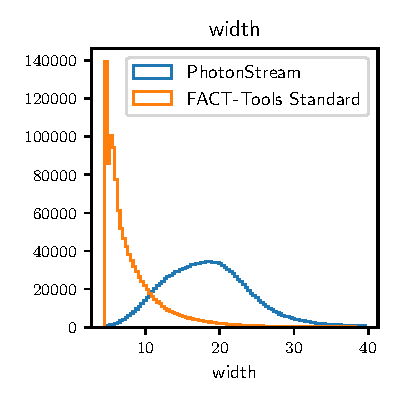
\includegraphics[width=\textwidth, page=1]{Plots/std_phs_comparison_hist_same_DBSCAN_crab.pdf}
  \end{subfigure}
  \begin{subfigure}{0.5\textwidth}
    \centering
    \includegraphics[width=\textwidth, page=2]{Plots/std_phs_comparison_hist_same_DBSCAN_crab.pdf}
  \end{subfigure}
  \begin{subfigure}{0.5\textwidth}
    \centering
    \includegraphics[width=\textwidth, page=3]{Plots/comparison_data_dl3.pdf}
  \end{subfigure}
  \begin{subfigure}{0.5\textwidth}
    \centering
    \includegraphics[width=\textwidth, page=4]{Plots/comparison_data_dl3.pdf}
  \end{subfigure}
  \caption{Hillas features for the same events on PhotonStream data and DBSCAN cleaning (blue) and on LP data and FACTtools cleaning (orange).}
  \label{fig:feat_comp}
\end{figure}
%
The direct comparison of the PhotonStream data's features illustrates the
differences of the cleaned air-showers: The air-shower's spatial features like
\texttt{width} and \texttt{length} are strongly shifted towards larger values.
From this it becomes clear that the DBSCAN cleaning is associating photons to
the shower cluster that lie within pixels far from the shower core, when
comparing to the classical cleaning. For the DBSCAN cleaning in the chosen
metric, photons that arrive in a close temporal proximity but within pixels not
containing large amounts of PE, can still easily be considered part of the
air-shower.

From these deviations another important question arises: how well do the MC
simualtions describe the reality or in other words do simulations and data
match as expected? Without knowing which photons within an event are air-shower
photons and which not it is hard to tell, whether the different topology of the
PhotonStream clusters is closer to the real air-shower or not.
\textbf{[Untersuchungen von Sebastian?]} Independent from that it is crucial to
have that same behaviour on simulations. \autoref{fig:feat_dbscan} shows the
distributions of \texttt{width}, \texttt{length} and \texttt{size} of
PhotonStream data on the DBSCAN cleaning for data and the gamma and proton MC
simulations.

The vast majority of the observed data is generally expected to be proton
events or other background. Therefore, the distributions of data and proton MC
should be more or less similar.
%
\begin{figure}
  \begin{subfigure}{0.5\textwidth}
    \centering
    \includegraphics[width=\textwidth, page=23]{Plots/data_mc/features_DBSCAN.pdf}
  \end{subfigure}
  \begin{subfigure}{0.5\textwidth}
    \centering
    \includegraphics[width=\textwidth, page=13]{Plots/data_mc/features_DBSCAN.pdf}
  \end{subfigure}
  \begin{subfigure}{0.5\textwidth}
    \centering
    \includegraphics[width=\textwidth, page=15]{Plots/data_mc/features_DBSCAN.pdf}
  \end{subfigure}
  \begin{subfigure}{0.5\textwidth}
    \centering
    \includegraphics[width=\textwidth, page=8]{Plots/data_mc/features_DBSCAN.pdf}
  \end{subfigure}
  \caption{Features using DBSCAN and standard parameters.}
  \label{fig:feat_dbscan}
\end{figure}

\begin{figure}
  \begin{subfigure}{0.5\textwidth}
    \includegraphics[width=\textwidth, page=23]{Plots/data_mc/features_DBSCAN_perc.pdf}
  \end{subfigure}
  \begin{subfigure}{0.5\textwidth}
    \includegraphics[width=\textwidth, page=13]{Plots/data_mc/features_DBSCAN_perc.pdf}
  \end{subfigure}
  \begin{subfigure}{0.5\textwidth}
    \includegraphics[width=\textwidth, page=15]{Plots/data_mc/features_DBSCAN_perc.pdf}
  \end{subfigure}
  \begin{subfigure}{0.5\textwidth}
    \includegraphics[width=\textwidth, page=8]{Plots/data_mc/features_DBSCAN_perc.pdf}
  \end{subfigure}
  \caption{Features using DBSCAN and additionally excluding pixels with less than $\SI{1}{\percent}$ PE of the air-shower's total \texttt{size}.}
  \label{fig:feat_dbscan_perc}
\end{figure}


\section{Time Features on the PhotonStream}
%
\begin{figure}
  \begin{subfigure}{\textwidth}
    \centering
    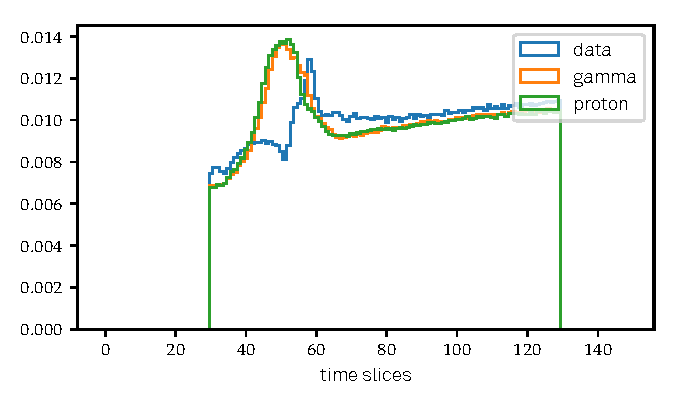
\includegraphics[width=0.8\textwidth]{Plots/all_slices_min_0_per_pixel.pdf}
  \end{subfigure}
  \begin{subfigure}{\textwidth}
    \centering
    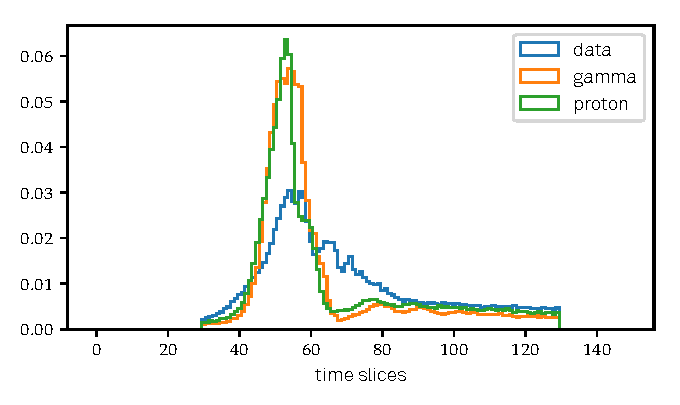
\includegraphics[width=0.8\textwidth]{Plots/all_slices_min_10_per_pixel.pdf}
  \end{subfigure}
  \caption{Arrival times of the single photons within all the pixels (top) and the cleaned air-shower pixels containing at least 10 photons (bottom) on data and MC simulations.}
  \label{fig:slices}
\end{figure}

\section{Origin Reconstruction}
%
As described in \autoref{sec:source_pos} the reconstruction of the source
position uses the air-shower's features \texttt{delta}, \texttt{width} and
\texttt{length}. The calculated angle \texttt{delta} plays a major role in
finding the right source position, since it describes the axis along which
the source position is assumed to be. It is calculated as the angle between
the shower's main axis and the camera's $x$-axis. Therefore, it is dependant
on the covariance of the light distribution and thus affected by the
differences within the PhotonStream.

To investigate the differences on PhotonStream data, it is possible to
calculate a true delta on the data images by using the telescope's pointing
position. From the pointing position and the known source position an
expected source position within the camera can be calculated. The
air-shower's cog and the calculated source position within the camera can
then be used to calculate a vector representing the estimated shower axis.
The calculated angle $\delta_\text{true}$ of that shower axis can thus be
compared to the calculated angle of the cleaned air-shower's main axis. The
distribution of these differences is expected to have two peaks: one around
zero and one around a difference of $\pi$. These two peaks correspond to
air-showers with a very small difference in $\delta$ and on the one hand the
right estimated sign of \texttt{disp} (zero) and on the other hand the
opposite estimated sign of \texttt{disp} ($\pi$). When dividing the
distribution into the different signs of \texttt{disp} there should only be
one peak for each distribution for a working sign classifier.

\autoref{fig:delta_fact} shows a distribution of $\symup{\Delta}\delta$ for
the pixel based cleaning as described in \autoref{sec:thresh} on LP data.
The two histograms represent the different estimations of the sign of
\texttt{disp} for the whole open data sample. The distributions show very
good agreement with the expectations described above. While this is not a
comparison with any real truth, it nevertheless shows a working
reconstruction of the air-shower events.
%
\begin{figure}
  \centering
  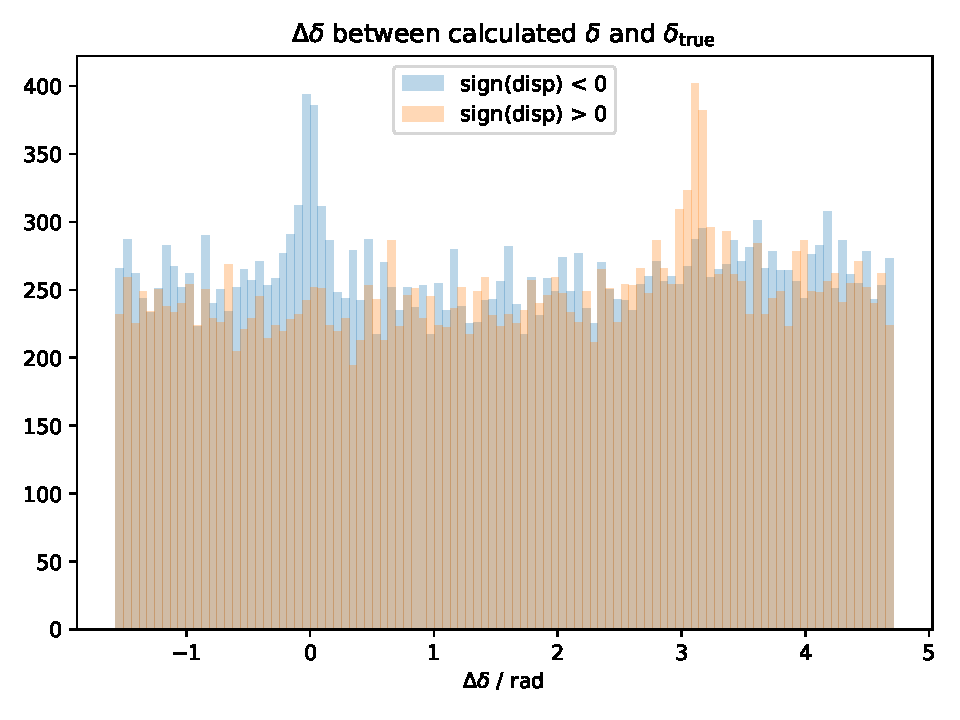
\includegraphics[width=0.7\textwidth]{Plots/delta_delta/delta_delta_facttools.pdf}
  \caption{Difference between calculated delta and true delta for the FACTtools analysis. The distributions show the calculated $\symup{\Delta}\delta$ for the different predictions of sign of \texttt{disp} on the whole open data crab sample.}
  \label{fig:delta_fact}
\end{figure}
%
When calculating $\symup{\Delta}\delta$ on the cleaned PhotonStream data, a
very different picture emerges. \autoref{fig:delta_diff_a} shows
$\symup{\Delta}\delta$ for the DBSCAN cleaning, when projecting the found
photons back to the camera plane and calculating \texttt{delta}. There are
hardly any peaks in these distributions, but rather widely spread
accumulation ranges around zero and $\pi$. Thus, the calculated
\texttt{delta} seems to differ quite sicnificantly from the expected
\texttt{delta}. Furthermore, both \texttt{sign} predictions show similar
distributions, hinting at a low accuracy for the \texttt{sign}
classification. The main differrence between the air-showers found by DBSCAN
and the ones found by the classic cleaning projected to the camera plane is
the spread across the camera axes. DBSCAN clustering is associating photons
from pixels quite distant from the shower core to the air-shower cluster.
This way, the spread within $x$ and $y$ becomes way bigger. Because
\texttt{delta} is calculated on the $x$-$y$-distribution weighted by the
number of photons, these outlier photons might have a big impact on the
calculation of \texttt{delta}, even though they usually only contain very
few photons. To prevent this from happening, the cleaning can be extended by
a step excluding pixels with less than $\SI{1}{\percent}$ of the total
amount of photons from the calculations of \texttt{delta}, \texttt{length}
and \texttt{width}. The distributions of $\symup{\Delta}\delta$ for this
cleaning are shown in \autoref{fig:delta_diff_perc}.

\begin{figure}
  \subcaptionbox{\label{fig:delta_diff_a}}[0.48\textwidth]{
    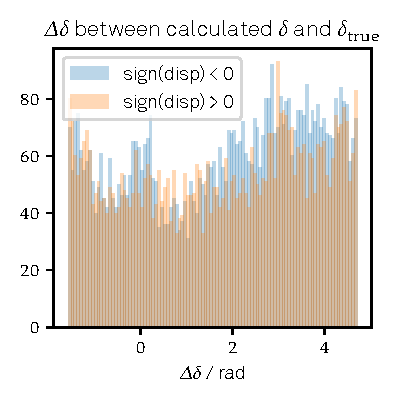
\includegraphics[width=0.5\textwidth]{Plots/delta_delta/delta_true_diff_hist_thresholds_rad_20131104_162.pdf}
  }
  \subcaptionbox{\label{fig:delta_diff_perc}}[0.48\textwidth]{
    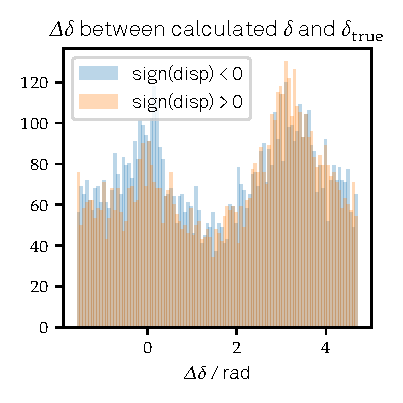
\includegraphics[width=0.5\textwidth]{Plots/delta_delta/delta_delta _DBSCAN_1perc_rad_20131104_162.pdf}
  }
  \caption{Difference between calculated delta and true delta for a subset of 500 data events. delta is calculated using all cleaned pixels \protect\subref{fig:delta_diff_a} and using only cleaned pixels containing more than $\SI{1}{\percent}$ of the air-shower's size \protect\subref{fig:delta_diff_perc}.}
  \label{fig:true_delta}
\end{figure}
%
The distributions change significantly, when adapting the cleaning.
The two peaks become quite distinctive around $0$ and $\pi$. Also the
different sign predictions show different heights around the two
accumulation points corresponding to the rightly classified signs, although
there seem to be frequent misclassifications. Although the results still
differ strongly from the ones shown in \autoref{fig:delta_fact}, the
accuracy of delta improves when neglecting outlying pixels. Thus, there
seems to be an impact of the large spread of DBSCAN clusters which is very
likely to also affect the origin reconstruction on such events.

%
\begin{figure}
  \begin{subfigure}{\textwidth}
    \centering
    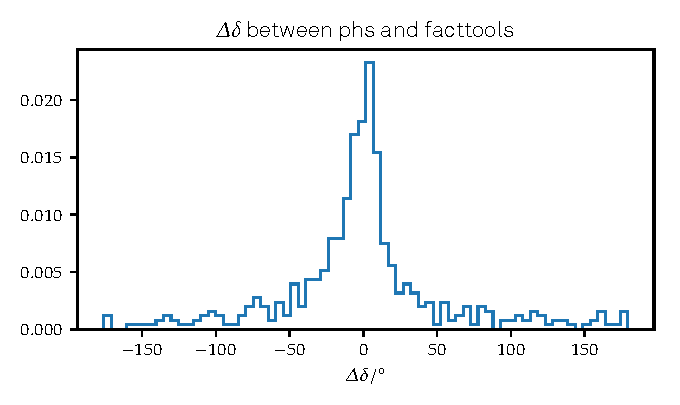
\includegraphics[width=0.8\textwidth]{Plots/delta_delta/delta_diff_hist_different_cleanings_DBSCAN_delta_20131104_162.pdf}
  \end{subfigure}
  \begin{subfigure}{\textwidth}
    \centering
    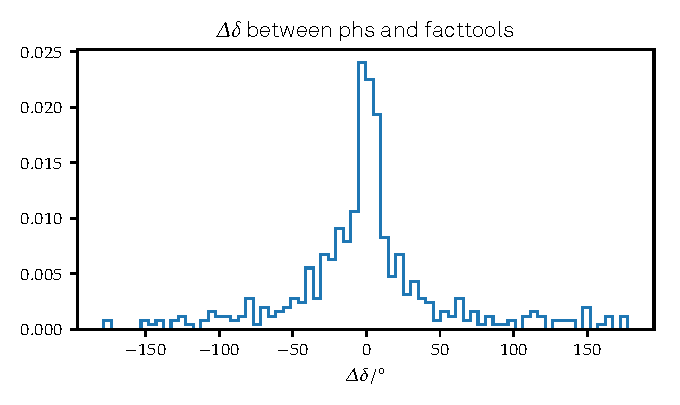
\includegraphics[width=0.8\textwidth]{Plots/delta_delta/delta_diff_hist_perc_DBSCAN_delta_20131104_162.pdf}
  \end{subfigure}
  \caption{Differences between the PhotonStream \texttt{delta} and the FACTtools \texttt{delta} for the DBSCAN cleaning (top histogram) and the DBSCAN cleaning extended by excluding pixels with less than $\SI{1}{\percent}$ of the shower's \texttt{size}.}
  \label{fig:delta}
\end{figure}
%
Since the FACTtools analysis yields good results and a working origin
reconstruction, the differences between its features and the DBSCAN cluster
features can also be investigated to understand the new data representation.
\autoref{fig:delta} shows the differences between the PhotonStream
\texttt{delta} and the FACTtools \texttt{delta} for the DBSCAN cleaning (top
histogram) and the DBSCAN cleaning extended by excluding pixels with less
than $\SI{1}{\percent}$ of the shower's \texttt{size}.
From these distributions, it becomes clear that the difference of the
PhotonStream's air-showers does not solely result from the wider spread of
the light distribution over the camera pixels. The two distributions barely
differ from another, although as shown by \autoref{fig:delta_diff_perc}, the
reconstruction of \texttt{delta} seems to improve with the additional
cleaning. For the majority of events the calculated \texttt{delta} is within
$\mathcal{O}(\SI{10}{\degree})$ to the FACTtools \texttt{delta}, but for the
origin reconstruction such a difference can become a difficult obstacle.
However, this comparison, as the one with the expected source position
within the camera, is not a comparison with truth values, but rather one
with a working analysis.

All these investigations, of course, serve the sole purpose of understanding
the different prerequisites for reconstructing the source position on
air-shower images. As described in \autoref{sec:source_pos} this is done by
using the \texttt{disp} method on Hillas parametrized images. Random forests
are used to estimate $|\texttt{disp}|$ via a regression task and then determine
the $\text{sign}(\texttt{disp})$ via a classification. The used random forests
consist of \num{100} estimators, each of which has a maximum depth of \num{15}.

The output of these random forests can then be projected from the air-shower's
core within the camera to sky coordinates, resembling the estimated source
position. Since the Crab Nebula is a well known source with a well known
position, the difference between the reconstructed and the knwon source
position can be calculated. It is tipically quantized as the euklidian distance
squared in $[\theta^2] = \si{\degree\squared}$ and illustrated as shown in
\autoref{fig:theta2}. These $\theta^2$-plots show the distribution of the
distances squared of the reconstructed source position per event from the Crab
Nebula's known position. They contain all events after preselection cuts and
applying the gamma hadron separation at a specific \texttt{gamma\_prediction}
threshold. The blue bins show the reconstructed signal events (On events) while
the orange bins represent the reconstructed background events (Off events). The
$\theta^2$-cut

For a Crab Nebula data sample and a working analysis the $\theta^2$-plot is expected to
%
\begin{figure}
  \begin{subfigure}{\textwidth}
    \centering
    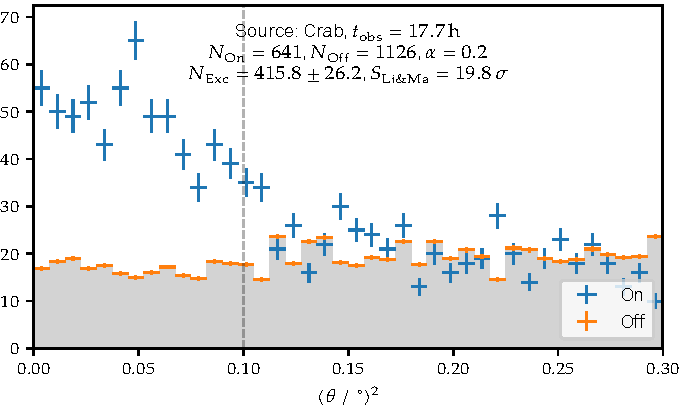
\includegraphics[width=\textwidth]{Plots/results/DBSCAN/theta2_plot.pdf}
  \end{subfigure}
  \begin{subfigure}{\textwidth}
    \centering
    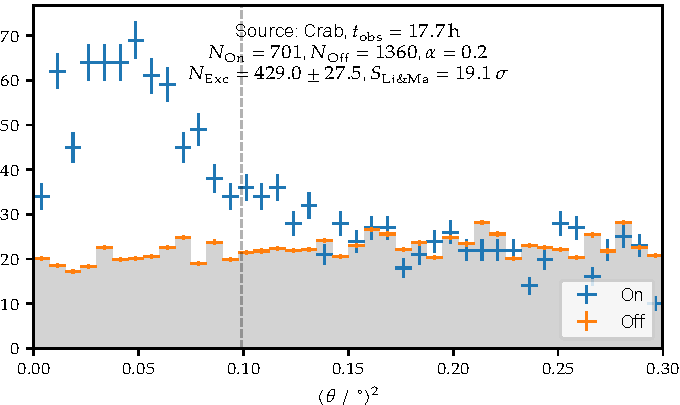
\includegraphics[width=\textwidth]{Plots/results/DBSCAN_perc/theta2_plot.pdf}
  \end{subfigure}
  \caption{$\theta^2$-plots for the PhotonStream data and dedicated analysis. The distributions of the distances squared of the reconstructed source position per event from the Crab Nebula's known position are shown. They contain all events after preselection cuts and applying the gamma hadron separation at a specific \texttt{gamma\_prediction} threshold. The blue bins show the reconstructed signal events (On events) while the orange bins represent the reconstructed background events (Off events).}
  \label{fig:theta2}
\end{figure}
%
\section{Energy Estimation}
%
%
\begin{figure}
  \centering
  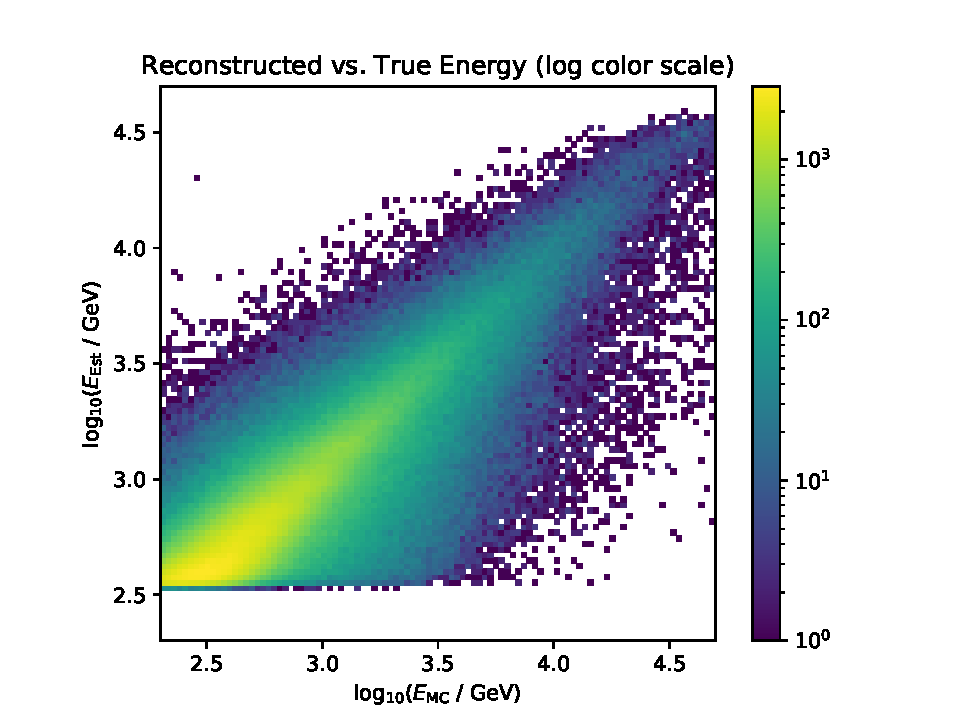
\includegraphics[width=0.8\textwidth, page=1]{Plots/results/DBSCAN/energy_performance.pdf}
  \caption{Energy estimation.}
  \label{fig:energy1}
\end{figure}
%
%
\begin{figure}
  \centering
  \includegraphics[width=0.8\textwidth, page=3]{Plots/results/DBSCAN/energy_performance.pdf}
  \caption{Energy estimation 2.}
  \label{fig:energy2}
\end{figure}
%
%
\begin{figure}
  \centering
  \includegraphics[width=0.8\textwidth, page=4]{Plots/results/DBSCAN/energy_performance.pdf}
  \caption{Energy estimation 3.}
  \label{fig:energy3}
\end{figure}
%

\section{Gamma Hadron Separation}
%
%
\begin{figure}
  \centering
  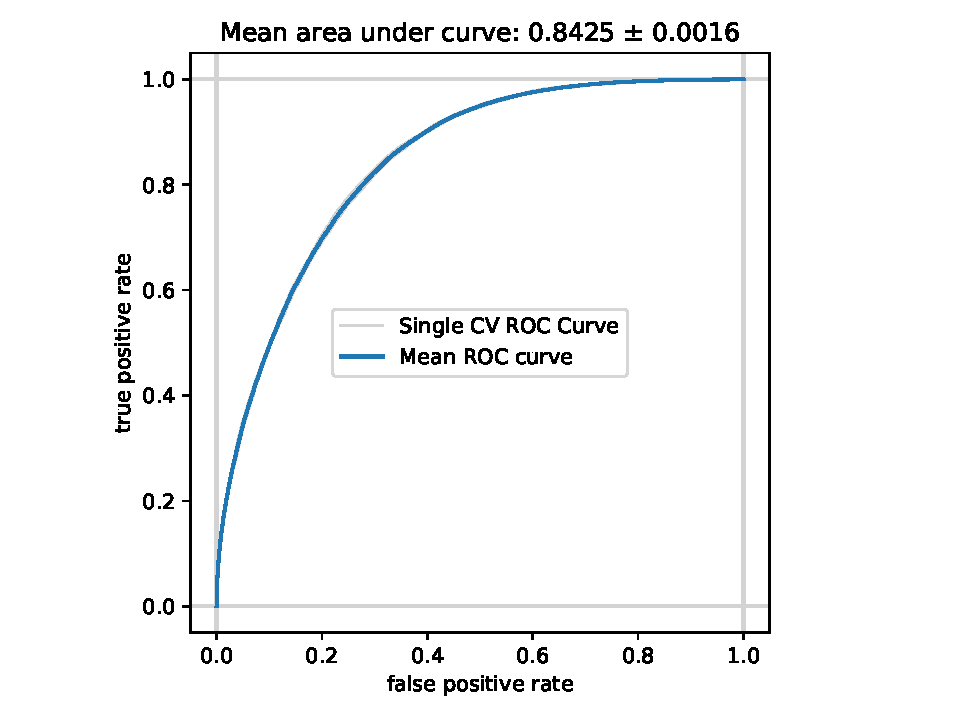
\includegraphics[width=0.8\textwidth, page=1]{Plots/results/DBSCAN/separation_performance.pdf}
  \caption{Gamma hadron separation.}
  \label{fig:sep1}
\end{figure}
%
%
\begin{figure}
  \centering
  \includegraphics[width=0.8\textwidth, page=3]{Plots/results/DBSCAN/separation_performance.pdf}
  \caption{Gamma hadron separation 2.}
  \label{fig:sep2}
\end{figure}
%
%
\begin{figure}
  \centering
  \includegraphics[width=0.8\textwidth, page=4]{Plots/results/DBSCAN/separation_performance.pdf}
  \caption{Gamma hadron separation 3.}
  \label{fig:sep3}
\end{figure}
%



\section{Parameters of DBSCAN}
%
\begin{figure}
  \centering
  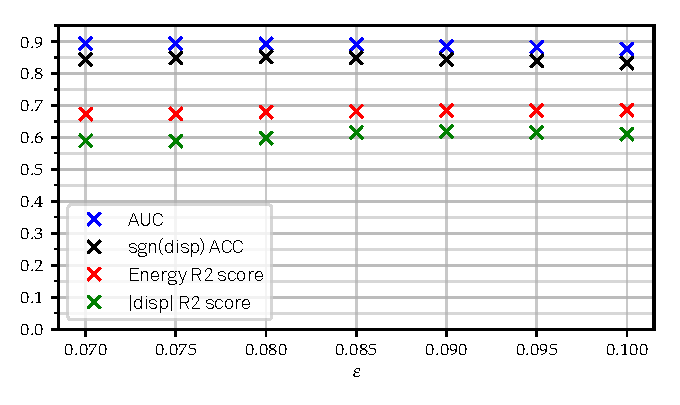
\includegraphics[width=0.7\textwidth]{Plots/Epsilon/eps_scores.pdf}
  \caption{Scores.}
  \label{fig:eps_scores}
\end{figure}
%
\begin{figure}
  \centering
  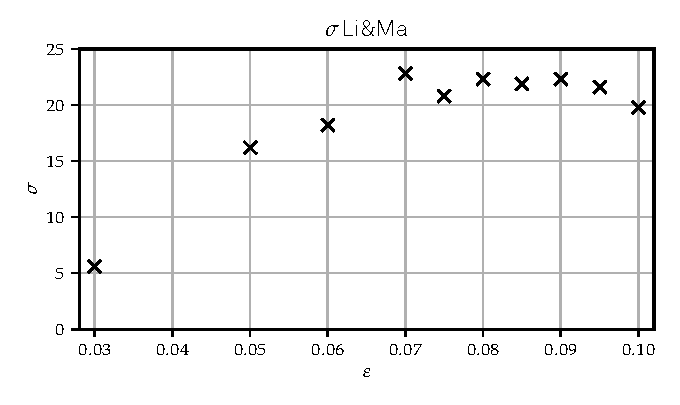
\includegraphics[width=0.7\textwidth]{Plots/Epsilon/eps_sigma.pdf}
  \caption{Detection significance.}
  \label{fig:eps_sigma}
\end{figure}
%
\begin{figure}
  \centering
  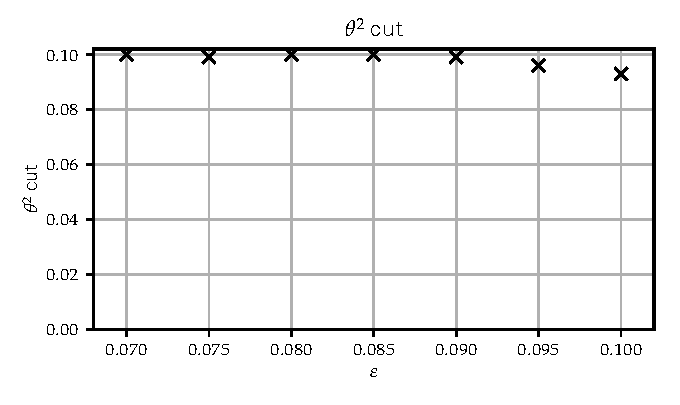
\includegraphics[width=0.7\textwidth]{Plots/Epsilon/eps_theta_cut.pdf}
  \caption{Detection $\theta^2$ cuts.}
  \label{fig:eps_theta}
\end{figure}

\section{Pixelbased Threshold Cleaning on the PhotonStream}
%
